\chapter{Verwandte Arbeiten}


In diesem Kapitel werden einige wissenschaftlichen Arbeiten vorgestellt,
auf denen diese Bachelorarbeit aufbaut.

\citeauthor{SHEWCHUK:2002:chuws} diskutiert ausführlich die Delaunay-Triangulierung und verschiedene Delaunay-Refinement Algorithmen in der euklidischen Ebene. Eine ausführliche Beschreibung des Delaunay-Refinement ist in Kapitel \ref{kap:Algorithmus} S.\pageref{kap:Algorithmus} dieser Bachelorarbeit zu finden.
In seinen Arbeiten werden auch die bekanntesten Verfahren von \citet{chew:1993:guaranteed,chew:1989:guaranteed} und \citet{ruppert:1995:delaunay} vorgestellt.
Da die Triangulierungen von geschlossenen StF-Oberflächen keine Segmente enthält, wird in dieser Bachelorarbeit nicht weiter auf den Unterschied der beiden Algorithmen eingegangen. Siehe dazu und zum jeweiligen Umgang mit Segmenten: \citeauthor{shewchuk:1997:delaunay}.\\
\begin{figure}[h]%{r}{5cm}
    \centering
  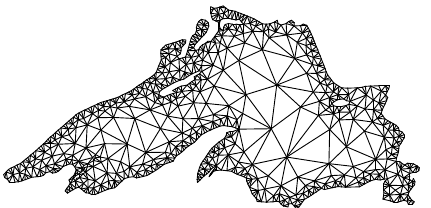
\includegraphics[width=3in]{images/tripslg.png}
  %\setcapindent{0em}
  \caption{Illustration des Delaunay-Refinement:
  Für das abgebildete Polygonzug erzeugt Chew zweite und Ruperts Version fast die gleiche Ausgangstriangulierung\cite{SHEWCHUK:2002:chuws}.}
\end{figure} 

Analog zur Triangulierung von Flächen in der euklidischen Ebene beschäftigen wir uns mit der Triangulierung \cite{Bobenko:2007:LaplaceBeltrami} von Flächen, die im dreidimensionalen Raum eingebettet sind. Diese werden in der Mathematik  vereinfachte als stückchenweise flache 2-Mannigfaltigkeiten  \cite{betke:1984:2-Mannigfaltigkeiten} bezeichnet.
\citeauthor{SHEWCHUK:2002:chuws} vermutet dazu, dass sich die Lemmata, welche für Triangulierungen gelten, übertragen lassen \cite[abschnitte 5.3.2]{SHEWCHUK:2002:chuws}. Diese Übertragbarkeit werden wir in Kapitel \ref{kap:Terminierung}  auch für einige Lemmata von \citet{ruppert:1995:delaunay} zeigen.\\  

Diese Arbeit orientiert sich an der Definition von \citet{Bobenko:2007:LaplaceBeltrami}, die auf den Arbeiten  \cite{boris1934delaunay,indermitte:2001:voronoi,lambert:1994:delaunay} aufbaut. Sie zeigen in ihrer Arbeit, dass die Eigenschaften, die für die Delaunay-Triangulierung in der Ebene gelten, sich auch auf die Delaunay-Triangulierung  von stückchenweise flachen Oberflächen \cite[Definiton 1] {Bobenko:2007:LaplaceBeltrami}  im dreidimensionalen Raum übertragen lassen \cite[Definition 3]{Bobenko:2007:LaplaceBeltrami}.\\

Von \citet{Bobenko:2007:LaplaceBeltrami} inspiriert entwickeln \citet{Bobenko:2006:SIGGRAPH} das \textit{incremental overlay-Schema} \cite[Abschnitt 2.3]{Bobenko:2006:SIGGRAPH}. Das Schema basiert auf dem expliziten Speichern von Kantenschnittpunkten und ist die erste Datenstruktur zur Realisierung intrinsischer Triangulierungen. Das \textit{incremental overlay-Schema} wurde gezielt für intrinsische Kantenflips entwickelt und unterstützt darüber hinaus nur wenige weitere Operationen \cite[Abschnitt 2]{Sharp:2019:NIT}. \\
\begin{figure}[h]%{r}{5cm}
    \centering
  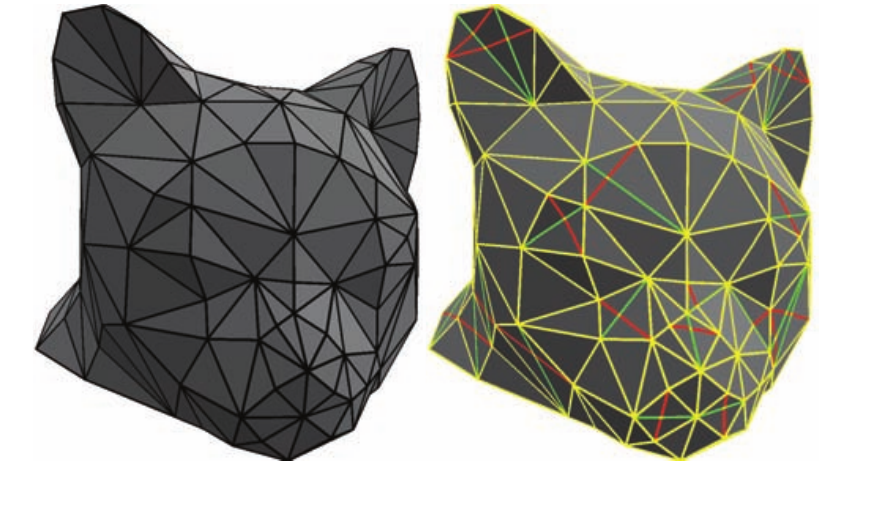
\includegraphics[width=3in]{images/overlaySchema.png}
  %\setcapindent{0em}
  \caption{Illustration des \textit{incremental overlay-Schema}:  Original kanten \textcolor{green}{grüne} geflipte Kanten \textcolor{red}{rot} und nicht veränderte kanten \colorbox{gray}{\textcolor{yellow}{gelb}}. Gespeichert werden die Schnittpunkte der Kanten.  \cite{Bobenko:2006:SIGGRAPH}}
\end{figure}
    
\citet{Sharp:2019:NIT} hat mit der \textit{signpost data structure} eine allgemeinere Datenstruktur vorgestellt \cite[abschnitt 3]{Sharp:2019:NIT}, welche weitere Operationen auf intrinsischen Triangulierungen ermöglicht. Mithilfe dieser Datenstruktur gelingt es ihm unter anderem, eine intrinsische Version des Delaunay-Refinement Verfahrens für Triangulierungen in der euklidischen Ebene auf Triangulierungen von stückchenweise flachen Oberflächen \cite[Definition 1]{Bobenko:2007:LaplaceBeltrami} anzuwenden. 
 \begin{figure}[h]%{r}{5cm}
    \centering
  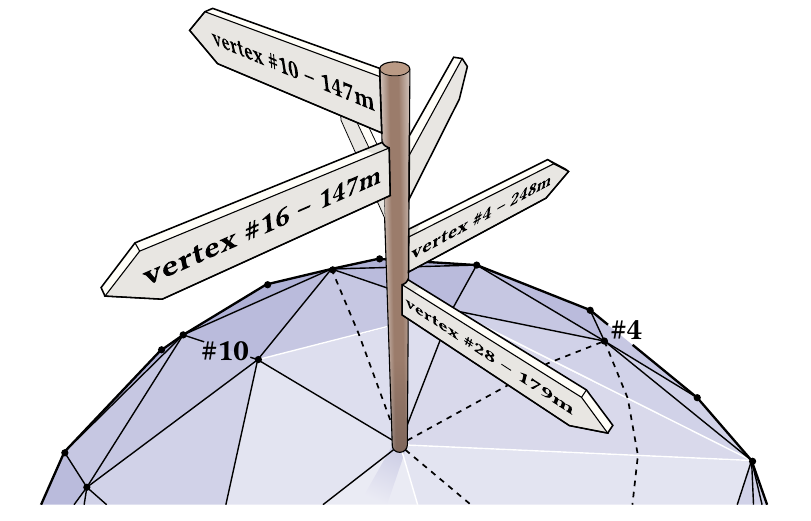
\includegraphics[width=3in]{images/signpostDataStructure.png}
  %\setcapindent{0em}
  \caption{Illustration des \textit{signpost data structure}: Sie basiert auf einer Halbkanten-Datenstruktur \cite{mantyla:1987:halfedge}, die  Triangulierungen implizit codiert, indem sie die Richtung und den Abstand benachbarter Knoten speichert. Diese implizite Codierung ermöglicht die praktische Anwendung des intrinsischen Delaunay-Refinement.  \cite{Bobenko:2006:SIGGRAPH}}
\end{figure}
Das intrinsische Delaunay-Refinement von \citeauthor{Sharp:2019:NIT} basiert auf dem zweiten Algorithmus von \citet{chew:1993:guaranteed}, mit der Modifikation, dass Dreiecke, die einen Knoten von Grad Eins enthalten, ignoriert werden. 
Da \cite{Sharp:2019:NIT} zur Unterstützung seiner These nur eine empirische Betrachtung vornimmt, ist noch nicht gesichert, dass der Algorithmus mathematisch korrekt ist und für jede Eingabe terminiert. Diese Bachelorarbeit beschäftigt sich daher mit dem Beweis, dass das intrinsische Delaunay-Refinement terminiert.\\

Es folgen nun weitere Möglichkeiten für Refinement-Verfahren, welche jedoch nicht Teil dieser Bachelorarbeit sind.

\citet{ungoe:2004:off-center} stellt das Delaunay-Refinement mit \textit{off-center}-Einfügestrategie vor, die eine Verallgemeinerung der Umkreismittelpunkt-Einfügestrategie ist.

\citet{rand:2011:Miller-Pav-Walkington} zeigte bereits mithilfe der \textit{Miller-Pav-Walkington analysis}, dass im zweidimensionalen Raum bessere Ergebnisse erzielt werden als mit dem bekannten Delaunay-Refinement.
Weitere Möglichkeiten hierfür sind auch die optimale Delaunay-Triangulierung von Chen und Xu \cite{chen:2004:mesh-odt,chen:2004:optimal-delaunay-triangulation} und die Minimal-Gewichtete-Triangulierungen von \citet{mulzer:2008:minimum}.

Die genannten Algorithmen ließen sich mit der von \citet{Sharp:2019:NIT} vorgestellten Datenstruktur auch leicht in eine intrinsische Form bringen.\\

Der Vollständigkeit halber werden an dieser Stelle noch andere Arbeiten genannt, die sich mit alternativen intrinsischen \textit{remeshing} beschäftigt haben. \citet{liu:2017:geodesic_Voronoi} und \citet{xin:2011:geodesic_delaunay} haben die intrinsische Delaunay-Triangulierung mithilfe  geodätischer Methoden erzeugt. Der Vorteil dieser Methode ist, dass die Ausgabe eine extrinsisches Triangulierung ist. Der Nachteil ist laut \citet{Sharp:2019:NIT}, dass unter Umständen viele Elemente erzeugt werden können und die Triangulierung zwar Delaunay-Eigenschaften hat, jedoch immer noch kleine Winkel aufweisen kann.\\ %Alt: 